\documentclass[10pt,twocolumn]{article}
\usepackage{paper-style}
\author{Francis Du}
\hypersetup{pdfauthor={Francis Du},pdftitle={WCode: Revision-Bound Evidence for Stateful Software Agents},pdfsubject={Software engineering runtime and evidence applicability}}
\begin{document}
\paperheading{WCode: Revision-Bound Evidence\\for Stateful Software Agents}{6 November 2026}{%
Software agents operate through sequences of repository reads, edits, checks, and acceptance decisions. Evidence produced at one step can become inapplicable after a code or design change, and a successful check from one producer can obscure a conflicting result from another. We present \wcode{}, a Rust runtime that makes these boundaries explicit. Its central abstraction is revision-bound evidence: observations retain their subject, producer, authority, coverage, and code--design revision, while policy determines whether they can support a current operation. The runtime combines bounded source delivery, optimistic file mutation, verification reuse, and producer-aware reconciliation. We specify the resulting admission contract and examine its implementation using a frozen executable. A model-free diagnostic covers 60 synthetic scenarios in four languages, three response budgets, two harness-cache phases, and seven repetitions, yielding 2,520 measured queries. Twenty-two selected contract counterexamples replay successfully on that same executable, and eleven operational controls pass. Every diagnostic condition delivers all 686 required source instances and all 406 eligible editing inputs. Nevertheless, serialized decision-record exposure varies from 0\% to 70\%, and removing writability from a readiness predicate creates seven false positives among 413 answerable observations per condition. The results show why successful retrieval and readiness for action need separate measurements. They support the tested runtime contracts; generalization to real-repository issue resolution remains an empirical question.}
\section{Introduction}
\label{sec:introduction}
Repository-level software agents increasingly combine code search, editing, command execution, and feedback within one workflow. SWE-bench measures the ability of complete systems to resolve real repository issues, while SWE-agent and OpenHands demonstrate the importance of the interfaces and execution environments surrounding a language model \cite{jimenez2024swebench,yang2024sweagent,wang2025openhands}. These systems make a second question consequential: when an agent acts on a previously observed result, what connects that result to the software state being changed?

Consider an agent modifying session-refresh behavior. It locates the correct function and obtains its source. Another worker then updates the same file. A test result remains available from the earlier revision, a second verifier reports a pass for a narrower target, and the implementation task is marked complete. None of these observations is necessarily false. The error arises if their distinct meanings are collapsed into a single indication that the current change is ready. Localization does not establish that an edit's source is current; an executed check does not establish coverage of every requirement; task completion does not establish acceptance.

This paper studies that coordination problem at the runtime boundary. We use \emph{evidence} to mean a typed observation about an artifact or operation, with recorded provenance and conditions of applicability. Evidence may remain useful as history after it ceases to justify a current operation. The key distinction is therefore between retaining an observation and admitting it into a present decision. This distinction matters whenever an agent, a human editor, and background checks share evolving software state.

We present \wcode{}, an implemented Rust runtime exposed through the Model Context Protocol. It maintains declared software intent, code observations, verification records, and work state. Its organizing rule is that an operation consumes evidence with explicit applicability conditions. Reading returns original source and file identity; mutation checks the current file against the observed identity; verification records the revision and authority under which a check ran; reconciliation preserves relevant disagreements between producers. The same rule also determines what the interface reports as missing or uncertain.

The research question is: \emph{How can a shared software-agent runtime preserve the applicability of evidence across bounded observation, concurrent modification, and verification?} We examine it through three contributions:
\begin{enumerate}
\item An explicit admission contract relating evidence to code--design revision, target scope, authority, and policy. The contract distinguishes current support, historical observations, and unresolved producer conflicts.
\item A runtime implementation that carries these distinctions across context packing, guarded single-file edits, verification execution and reuse, and reconciliation. A running example shows why preserving the fields at each boundary is necessary.
\item An auditable diagnostic evaluation separating source delivery, edit-input readiness, operational controls, and descriptive cost. A retained executable and source archive identify the primary run; a predicate-removal analysis exposes a readiness error hidden by saturated retrieval scores.
\end{enumerate}

The contribution is a composition of established mechanisms around a shared operational contract. Hashing, provenance, architecture conformance, and access control each have substantial prior work; Section~\ref{sec:related} locates the runtime within those traditions. Our evaluation is correspondingly specific. It invokes no language model and establishes behavior on developer-authored scenarios rather than improved patch success. This scope allows us to inspect failures at tool boundaries without attributing them to model reasoning, while leaving downstream effectiveness to a separate experiment.

\section{An Evidence Admission Contract}
\label{sec:contract}
\subsection{State and observations}
Let the workspace state be
\begin{equation}
 S=(D,C,P,G,E,W),
\end{equation}
where $D$ is declared design, $C$ is code, $P$ is applicable policy, $G$ is the observed software graph, $E$ is the evidence history, and $W$ is work state. Its revision is $\rho(S)=(\rho_C,\rho_D)$, with an optional design component. Policy has a separate binding; it is not a third revision field. Keeping design in the revision matters because a changed acceptance criterion can invalidate the use of a previous result even when the code bytes are unchanged.

For exposition, represent an evidence record as
\begin{equation}
 e=(u,k,p,\rho,\sigma,a,o,\pi,\tau),
\end{equation}
where $u$ is the subject, $k$ the evidence kind, $p$ the producer, $\rho$ the captured revision, $\sigma$ the covered targets, $a$ the authority, $o$ the outcome, $\pi$ the relevant policy binding, and $\tau$ an ordering or execution receipt. This tuple summarizes checks distributed across the implementation; it is not a claim that every subsystem has one identical record schema.

Provenance and authority serve different purposes. A producer identifier records who supplied an observation. Authority determines which claims that entry point is allowed to establish. A self-reported producer name or confidence score cannot turn external evidence into native verification. Similarly, automated policy authorization and an explicit human approval are distinct evidence kinds. Replacing either distinction with a generic ``success'' would change the meaning of the decision.

\subsection{Applicability and producer conflicts}
For a request $q$, define the applicable subset
\begin{align}
 E_q(S)&=\{e\in E:\App(e,S,q)\},\\
 \App(e,S,q)&=\operatorname{Complete}(e.\rho) \nonumber\\
 &\quad\land(e.\rho=\rho(S)) \nonumber\\
 &\quad\land\operatorname{Relevant}(e.\sigma,q) \nonumber\\
 &\quad\land\operatorname{Authorized}(e.a,P,q) \nonumber\\
 &\quad\land\operatorname{Compatible}(e.\pi,P,q).
 \label{eq:applicable}
\end{align}
The predicates are operation-specific. Relevance admits observations about the request's targets; exact coverage is checked when a record supports an individual obligation. Compatibility concerns the policy conditions relevant to that evidence kind. An incomplete revision fingerprint cannot establish exact-revision native evidence. Retaining such a record for inspection does not make it applicable.

Applicability alone does not resolve conflicting records. We reduce records within keys that retain subject, evidence kind, producer, and applicability scope. A newer record can supersede an older one only under the applicable typed-receipt and coverage rules. Let $L_q$ denote the resulting retained records. A global ``latest result wins'' reduction is unsuitable: a pass from producer $p_2$ must not erase an applicable failure from $p_1$.

Let $Q$ be the nonempty set of required checks, $A$ the additional configured acceptance gates, and $\bar S=(D,C,P,G,W)$ the state excluding evidence history. A simplified admission rule is
\begin{align}
 \Accept(S,q) \iff{}& Q\ne\varnothing \nonumber\\
 &\land\ \forall t\in Q:\Pass(t,L_q) \nonumber\\
 &\land\ \nexists e\in L_q:\Fail_q(e) \nonumber\\
 &\land\ \operatorname{GatesSatisfied}(A,\bar S,L_q).
 \label{eq:accept}
\end{align}
Here, $\Pass(t,L_q)$ requires applicable support whose coverage, kind, authority, and receipt satisfy check $t$; an outstanding skipped check cannot supply it. $\Fail_q(e)$ denotes a blocking failure under the request's policy, rather than every negative or advisory observation. Configured gates consult evidence only through $L_q$. The implementation distinguishes check aggregation from broader reconciliation and acceptance. Equation~\eqref{eq:accept} makes their logical dependency explicit rather than replacing them with a single execution-status flag.

\begin{proposition}[Preservation under irrelevant additions]
\label{prop:preservation}
Fix $\bar S$, the request $q$, the required checks and gates, and the reduction rules. Adding inapplicable evidence does not change admission. If a retained applicable blocking failure from producer $p_1$ remains, adding a passing record from a different producer $p_2$ cannot make admission true.
\end{proposition}
\begin{proof}
Inapplicable records are removed before reduction and therefore leave $L_q$ unchanged. All other arguments to the checks and gates are fixed, so admission is unchanged. Records from distinct producers occupy distinct reduction keys, so the added pass cannot supersede the blocking failure. The failure makes the third conjunct of Equation~\eqref{eq:accept} false.
\end{proof}

The proposition concerns the specified admission rule under truthful, complete, correctly bound inputs. It does not establish that a test is adequate, that a producer is trustworthy, or that an implementation is formally verified. In particular, a captured revision label alone cannot prove that a process read an immutable snapshot throughout execution. These assumptions separate what the contract guarantees from what evidence capture must establish.

\subsection{A running change scenario}
Table~\ref{tab:trace} gives a schematic trace for the session-refresh example. The identifiers are illustrative, not an additional empirical task. The trace exposes two independent validity boundaries: the file observation used by an edit and the revision-bound support used by acceptance.

\begin{table}[t]
\small
\caption{Illustrative evidence transitions for one change.}
\label{tab:trace}
\begin{tabularx}{\columnwidth}{@{}p{0.19\columnwidth}X@{}}
\toprule
Event & Consequence for the next operation\\
\midrule
Read $h_0$ & The response identifies the function, original body, and current file hash.\\
Peer edits & File state becomes $h_1$; an edit still expecting $h_0$ must refresh its input.\\
Old pass & Evidence bound to $\rho_0$ remains historical when the current revision is $\rho_1$.\\
$p_1$ fails & A current failure remains visible for its subject and scope.\\
$p_2$ passes & A pass from another producer does not supersede $p_1$'s failure.\\
Task ends & Completion updates work state; acceptance still requires applicable checks and gates.\\
\bottomrule
\end{tabularx}
\end{table}

There is no universal ordering in which a source excerpt, a test pass, and a human approval are interchangeable amounts of confidence. They support different predicates. The runtime consequently exposes both the observations and the remaining obligations, allowing a caller to choose a targeted re-read, re-verification, or review instead of inferring readiness from an undifferentiated score.

\section{Runtime Design and Implementation}
\label{sec:implementation}
\wcode{} implements the contract through four connected responsibilities: observing software state, constructing bounded context, admitting mutations, and reconciling verification evidence. Figure~\ref{fig:architecture} shows their relationship. The runtime does not prescribe the caller's model or planning policy; it constrains the meaning of the operations available to that caller.

\begin{figure*}[t]
\centering
\begin{tikzpicture}[
  block/.style={draw=inkblue!75,rounded corners=2pt,align=center,inner sep=7pt,font=\small,text width=1.83in,minimum height=.55in},
  store/.style={block,fill=palegray},
  arr/.style={-{Latex[length=2mm]},line width=.6pt,draw=inkblue!90},
  note/.style={font=\footnotesize,fill=white,inner sep=2pt,align=center}]
\node[block] (context) {Bounded context\\identity, source, file hash};
\node[block,right=.44in of context] (edit) {Guarded mutation\\policy, lock, hash check};
\node[block,right=.44in of edit] (verify) {Verification\\execute, reuse, record};
\node[store,below=.64in of context] (state) {Software state\\design, code, observed graph};
\node[store,below=.64in of edit] (ledger) {Evidence history\\revision, producer, authority};
\node[block,below=.64in of verify] (reconcile) {Reconciliation\\coverage, conflicts, gates};
\draw[arr] (context) -- node[note,above]{edit inputs} (edit);
\draw[arr] (edit) -- node[note,above]{new revision} (verify);
\draw[arr] (state) -- node[note,left]{observe} (context);
\draw[arr] (edit.south west) -- node[note,above,sloped]{invalidate} (state.north east);
\draw[arr] (verify.south west) -- node[note,above,sloped]{receipts} (ledger.north east);
\draw[arr] (ledger) -- node[note,above]{applicable set} (reconcile);
\draw[arr] (state) -- node[note,above]{revision binding} (ledger);
\draw[arr] (verify) -- node[note,right]{outcomes} (reconcile);
\end{tikzpicture}
\caption{The runtime carries evidence across operation boundaries. Source identity constrains mutation; revision and provenance constrain verification reuse and reconciliation. The caller receives operation results and remaining obligations. Historical records remain inspectable after they lose applicability.}
\label{fig:architecture}
\end{figure*}

\subsection{Observing design and implementation}
Declared design represents requirements, components, constraints, decisions, and acceptance criteria. References connect components to files or symbols, and requirements to implementation and verification targets. These references provide traceability: resolving a symbol establishes a mapping, while behavior still requires appropriate verification.

The software graph joins declarations with files, symbols, tests, risks, and evidence. Observed relationships retain their provider, precision, and revision. Syntax-derived structure and fresh semantic-provider results therefore remain distinguishable. A bounded traversal reports incomplete coverage; ambiguous symbol matches or multiple component owners remain candidates. For architectural comparison, the absence of an observed edge is recorded as unverified actual structure when the observation is insufficient. It is not converted into a definite missing dependency.

Design admission is scoped to initialized product designs. In that setting, invalid design state or missing implementation ownership can block a mutation. The rule does not require every unrelated workspace to define a product model. This scope is important: applying a design gate without its initialization precondition would turn a useful project contract into an unexplained global prohibition.

\subsection{Observation surfaces over the same contract}
Operator surfaces are projections of the same recorded state rather than a parallel evidence store. The architecture workbench carries a design consistency view beside the system map, component, dependency and code graph surfaces. One row per requirement, component, acceptance check or constraint states the design intent, the observed state, and the delta between them. Dependency alignment keeps four evidence states apart: an unverified declared dependency is not missing implementation, and an undeclared observation is actionable only when its provider is stronger than syntax. Truncation and a zero denominator travel with the counts.

Every recorded drift is queued separately by the three existing kinds: implementation drift, design drift, and runtime drift. A finding carries its identifier, kind, risk, subject, message, affected requirements and paths; numeric drift additionally carries its metric, expected bound, observed value, unit, deviation, precision and revision binding. A finding is a prompt to confirm, not a verdict on the code. A truncated queue says so, the absence of a finding is not an all-clear, and runtime percentages are never combined with structural dependency percentages.

Investigation continuity keeps the operator's place. Switching the main view preserves the active filter, scroll position and selected object, while changing a filter re-selects the first visible item. A shareable link names the workspace, view, object and investigation label, so a copied link restores the object the operator was reading rather than an earlier selection. These are presentation guarantees over recorded state: they create no evidence, execute no check and grant no acceptance.

\subsection{Bounded context as an output contract}
The context interface assembles task targets, original source, file metadata, graph relationships, available checks, and work state. Selection prioritizes explicit targets and useful executable definitions; independent source items can be loaded concurrently. Packing then compacts reconstructible metadata and trims lower-priority content to satisfy an explicit response budget.

For serialized response $y$, the accounted size is
\begin{equation}
 b(y)=\left\lceil\frac{|\operatorname{JSON}(y)|_{\mathrm{bytes}}}{4}\right\rceil.
 \label{eq:budget}
\end{equation}
The requested bound is $b(y)\le B$. This byte-based proxy is an interface accounting rule, not a model tokenizer. A complete source window retains original content and line bounds; summaries do not stand in for missing original source. Readiness is refreshed after packing because a symbol found internally may be absent from the delivered response. Final serialization is checked against the budget, with an error if the bound cannot be met.

This output-centered design creates a testable invariant: readiness must be supported by what the caller actually receives. An internal retrieval hit cannot establish delivered-body coverage, and a current hash cannot compensate for an omitted body. Section~\ref{sec:results} evaluates these predicates separately.

\subsection{Optimistic mutation at a defined scope}
An existing-file mutation supplies an expected SHA-256 hash. Admission checks write policy, resolves the path, acquires its per-file lock, resolves the path again, rejects unsupported link conditions, and compares the current hash with the expected hash. The runtime validates the proposed content before an atomic single-file replacement and returns before/after hashes. Algorithm~\ref{alg:edit} abstracts this sequence.

\begin{algorithm}[t]
\small
\caption{Guarded edit admission (contract abstraction)}
\label{alg:edit}
\textbf{Input:} path $f$, observed hash $h$, requested edit $\Delta$\\
\textbf{Output:} committed hashes or a typed rejection
\begin{enumerate}[label=\arabic*.,leftmargin=1.6em]
\item Check applicable workspace, design, and write policy.
\item Resolve $f$ and acquire its per-file mutation lock.
\item Re-resolve $f$; validate path and link conditions.
\item Read current bytes $x$. If $\Hash(x)\ne h$, reject as stale.
\item Construct $x'=\Delta(x)$; validate edit preconditions and proposed content. Reject on failure.
\item Atomically replace the single file with $x'$; release the lock; return $\Hash(x),\Hash(x')$.
\end{enumerate}
The lock is released on every exit path. Independent files in a batch have independent outcomes.
\end{algorithm}

Under cooperating writes protected by this lock, two requests based on the same hash cannot both commit over successive byte-changing states: after the first changes the bytes, the second sees a different hash and fails its precondition. This consequence assumes the first write changes the hash and excludes a hash collision. A no-op write need not invalidate the second request. External editors need not cooperate with the lock, and the batch API is not a multi-file transaction. Callers must inspect partial outcomes and refresh after conflicts.

Command execution has a separate policy boundary. Permission to edit a file does not confer permission to launch an arbitrary process. Keeping file and process admission distinct makes rejection attributable to the relevant operation instead of silently widening authority.

\subsection{Verification and reconciliation}
Verification captures its input revision before executing a plan. Reports distinguish executed, reused, failed, and skipped checks. The aggregate execution pass requires at least one check, no failures, and no outstanding skipped checks. Eligible in-flight work can be coalesced for a matching revision, while each caller receives an explicit result. Reuse points to existing exact-revision evidence; it does not manufacture a new execution receipt.

Native recording rejects revision fingerprints marked as partial. Trusted entry points assign evidence authority. Producer-aware reduction retains relevant failures until the permitted supersession conditions are met. Consequently, a work item can be complete while its acceptance obligations remain unresolved.

Reconciliation connects declared changes, affected components, implementation tasks, verification plans, and acceptance gates. Its operator-facing state preserves missing mappings, conflicting results, and outstanding review. A design-only change can indicate implementation lag; a mapped code change without a design change can request review without asserting that every implementation-only refactoring is wrong. Runtime queue observations remain advisory when they lack source-revision binding. These distinctions prevent operational activity from being mistaken for accepted software.

\section{Evaluation Design}
\label{sec:evaluation}
We evaluate the implemented boundaries through four questions: (RQ1) do selected contract tests and operational controls preserve their stated boundaries; (RQ2) does bounded context deliver its annotated source obligations; (RQ3) which readiness errors are hidden by weaker predicates; and (RQ4) how do response size, visible decision records, and latency vary across the tested budgets? The unit under study is a runtime call, without a language-model invocation.

\subsection{Corpus and execution protocol}
The diagnostic contains 60 synthetic, developer-authored scenarios: 27 Rust and 11 each in Go, TypeScript, and Python. Fixtures range from 26 to 644 files. Each scenario has explicit Gold source obligations, including path-qualified identities and original source ranges. Among the 59 answerable scenarios, the union of required original source is small: 61--220 bytes per scenario, with a median of 162 bytes. One scenario is unanswerable and one is answerable but read-only; 58 are eligible for editing. These properties make the corpus useful for contract diagnostics but easy for source-delivery recall.

We run budgets $B\in\{1000,2000,4000\}$, two harness-cache phases, and seven repetitions per scenario and condition. This yields $60\times3\times2\times7=2520$ measured queries, plus 180 separate warm-up queries. ``Cold'' creates a new tool harness; ``warm'' uses its primed state. Operating-system caches are not cleared. Budget order is fixed, and phase order alternates by scenario. Repetition characterizes execution variability on the same tasks rather than creating new independent tasks.

The primary run uses an archived source tree at commit \code{584abd88}, package version 0.9.6, and a retained debug executable. It ran on an Apple M5 system with ten physical/logical cores and 16\,GiB memory, macOS 27.2 on arm64. The runtime toolchain probe reported rustc 1.99.1; it is not a separate attestation of the compilation toolchain. The harness is configured for four slots. Host load was not controlled. The complete source and executable identities, protocol, and recovery history are recorded in Appendix~\ref{sec:artifact} and the accompanying evidence inventory.

\subsection{Delivery and readiness measures}
For each condition, the 420 measured attempts contain 686 required source instances, 413 answerable observations, and 406 eligible editable observations. We score the following nested delivery predicates against the final response:
\begin{description}[style=unboxed,leftmargin=0pt,font=\bfseries]
\item[Identity.] The annotated path-qualified target is present.
\item[Original body.] The required source is delivered without truncation; this predicate already checks the source-window hash.
\item[File metadata.] The associated \code{files[]} entry also reports the current SHA-256.
\item[Editable input.] The response satisfies the complete editing-input contract, including write eligibility.
\end{description}
The first three source-instance measures use 686 obligations per condition; editable-input success uses 406 eligible observations. Separately, an attempt-level readiness analysis compares positive classifications among the 413 answerable observations. Keeping these denominators explicit prevents source recall from being reported as edit readiness.

We also measure the presence of a serialized \code{DecisionBatch}, an optional structured decision record in the final response. Its denominator is all 420 attempts. Exposure measures what the caller can inspect; it is not decision correctness. The raw report additionally retains shadow context-sufficiency scoring, which is a separate diagnostic and does not change the exposure measure.

\subsection{Controls, ablation, and timing}
Eleven operational controls cover four language-specific syntax graphs, guarded editing and invalidation, read-only admission, competing same-hash writes, workspace boundaries, partial-graph reporting, syntax-cache pressure, and workspace-relative verification singleflight. They exercise selected mechanisms alongside the primary trial.

We additionally replay 22 existing selected counterexample tests on the same retained executable, once per exact test name. They cover evidence identity and authority (11), producer conflict (2), dependency ownership (2), scope and observability (2), and scoring (5). Each invocation records its arguments, result, and before/after executable hashes. The source manifests and primary raw report are checked before and after the replay. Earlier executions under another build remain historical; the new replay supplies the results reported here.

The predicate analysis recombines retained per-sample score fields produced by grading the final responses; full serialized tool responses are not archived. It is an observational ablation of readiness definitions, not a runtime experiment that disables a module. For cost, we report serialized bytes and wall-clock latency of the context call. Timing excludes compilation, fixture construction, grading, model inference, network transport, and client retries. Table~\ref{tab:cost} summarizes all 420 observations per condition. Figure~\ref{fig:latency} instead plots 60 scenario medians, each formed from seven repetitions, so heavily repeated fixtures are not visually presented as independent tasks. We report descriptive distributions without inferential confidence intervals.

\section{Results}
\label{sec:results}
\subsection{Contract and operational boundaries}
All 22 selected counterexample tests pass when replayed individually on the same retained executable as the context diagnostic. Each invocation reports one passed test, zero failed tests, and zero ignored tests; none times out. Executable hashes match before and after every invocation, and the 774-path source manifest, all 1003 archived source files, and the primary raw report remain unchanged. Table~\ref{tab:counterexamples} groups the tested boundaries.

\begin{table}[t]
\small
\caption{Selected counterexamples replayed on the retained executable. Each test is executed once. Counts indicate successful expected behavior, not sampled failure-detection accuracy.}
\label{tab:counterexamples}
\begin{tabularx}{\columnwidth}{@{}Xr@{}}
\toprule
Boundary and tested distinction & Passed\\
\midrule
Acceptance: revision, receipt, authority, and approval conditions & 11/11\\
Producer conflict: applicable failures survive another producer's pass & 2/2\\
Dependency ownership: uncertain mappings remain qualified & 2/2\\
Scope and observability: unresolved work and verification state & 2/2\\
Evaluator: grading behavior on constructed counterexamples & 5/5\\
\midrule
Total & 22/22\\
\bottomrule
\end{tabularx}
\end{table}

These tests give concrete instances of the contract in Section~\ref{sec:contract}: a result with the wrong revision or authority cannot supply the required support, and a passing record from another producer does not remove an applicable blocking failure. The outcomes validate the selected assertions under the tested fixtures. They do not establish the adequacy of arbitrary verification plans or resistance to adaptive attacks. Earlier executions of these tests used a different build; the replay resolves that provenance difference without pooling the two executions.

All eleven primary controls pass. In the competing-write control, two operations begin with the same observed hash; one commits and one is rejected. The read-only and workspace-boundary controls reject their ineligible operations. Partial-graph reporting retains its incomplete status. Under syntax-cache pressure, the recorded run performs 13,168 trims and still reports 96 files, 96 matches, zero failures, and complete coverage. Workspace-relative verification singleflight passes its targeted duplicate-execution check.

These controls support RQ1 at their stated granularity. For example, the concurrent-write outcome is evidence for the guarded single-file path under the tested schedule. It does not establish transactional multi-file editing or coordination with every external process.

\subsection{Bounded source delivery}
For every budget--phase condition, identity, complete original-body delivery, and current file-metadata SHA each satisfy all 686 annotated obligations. All 406 eligible editing attempts satisfy the strict edit-input predicate. Across six conditions, this corresponds to 4116 required source instances and 2436 eligible editing attempts. There are no query errors, response-budget overruns, or warm-up errors.

These saturated outcomes answer RQ2 for the retained corpus. They also reveal the corpus's limited discrimination: its required source is small enough to fit even the lowest budget. A 100\% source score therefore says little about how additional budget changes other useful evidence. Figure~\ref{fig:budget} juxtaposes the saturated delivery measures with decision-record exposure and actual response size to make that distinction visible.

\begin{figure*}[t]
\centering
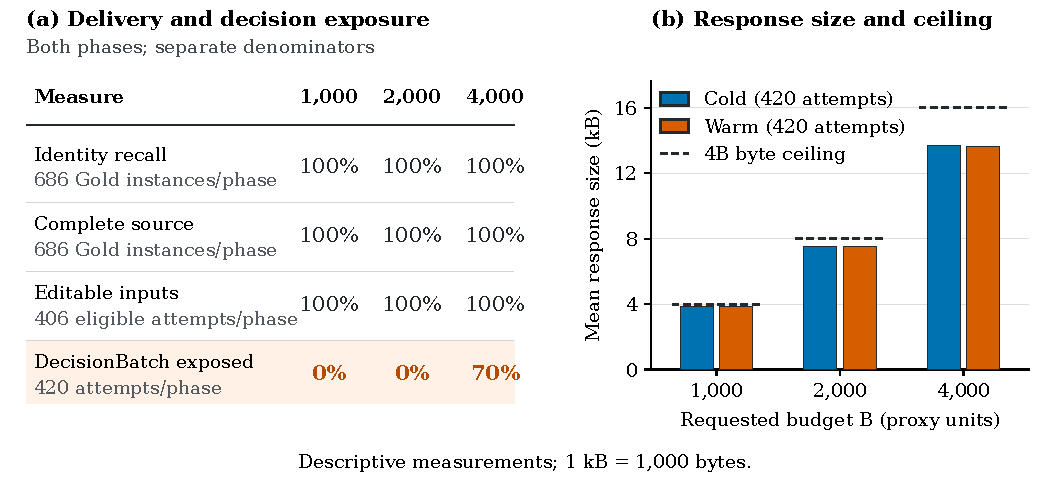
\includegraphics[width=\textwidth]{figures/budget_exposure.pdf}
\caption{Budget changes different outputs differently. Left: source delivery, editable-input success, and serialized decision-record exposure use distinct denominators (686 source obligations, 406 editable attempts, and 420 total attempts per condition). Rates agree between cold and warm phases; phases are not pooled. Right: mean serialized response bytes remain below the $4B$ ceiling implied by the accounting rule. The lowest budget already saturates the source-delivery measures.}
\label{fig:budget}
\end{figure*}

\subsection{Nested readiness predicates}
For RQ3, the attempt-level identity, body, and body-plus-file-metadata predicates each classify 413 answerable observations as positive per condition. The full editable-input predicate classifies 406. Omitting write eligibility therefore admits seven read-only observations, or $7/413=1.69\%$ of answerable observations. Across all six conditions, the 42 affected observations repeat the same read-only fixture; they are not 42 independently discovered vulnerabilities.

The result is small but diagnostic. Correct localization, original source, and fresh hashes can all be present while editing remains inadmissible. Removing the extra file-metadata SHA predicate produces no further separation in this corpus; the preceding body predicate already checks the source-window hash. The analysis therefore does not identify independent causal effects for each nested condition. It establishes a concrete counterexample to equating source availability with edit readiness.

\subsection{Budget, visibility, and latency}
Serialized \code{DecisionBatch} exposure is 0/420 at budgets 1000 and 2000, and 294/420 (70\%) at budget 4000, in both phases. Thus, equal source recall does not imply equal visibility into the runtime's structured decisions. This finding answers the visibility part of RQ4 without interpreting the exposed records as correct decisions on real tasks.

\begin{table*}[t]
\centering\small
\caption{Descriptive cost of the frozen primary run. Each row contains 420 measured calls. Latency quantiles summarize calls; the ECDF in Figure~\ref{fig:latency} uses scenario medians instead. Bytes are serialized JSON bytes, not model tokens.}
\label{tab:cost}
\begin{tabular}{@{}rrcrrrr@{}}
\toprule
Budget $B$ & Byte ceiling $4B$ & Phase & Mean bytes & p50 (ms) & p95 (ms) & Decision exposure\\
\midrule
1000 & 4000 & Cold & 3850.14 & 40.186 & 70.913 & 0/420\\
1000 & 4000 & Warm & 3849.71 & 27.030 & 51.216 & 0/420\\
2000 & 8000 & Cold & 7506.04 & 34.795 & 61.286 & 0/420\\
2000 & 8000 & Warm & 7503.97 & 20.738 & 34.736 & 0/420\\
4000 & 16000 & Cold & 13667.22 & 25.709 & 56.378 & 294/420\\
4000 & 16000 & Warm & 13663.93 & 12.948 & 25.150 & 294/420\\
\bottomrule
\end{tabular}
\end{table*}

\begin{figure}[t]
\centering
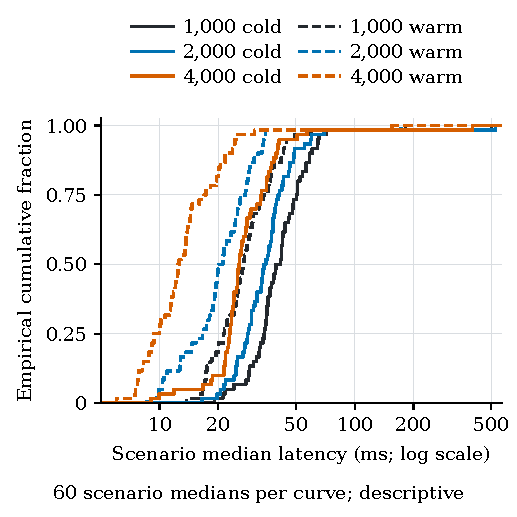
\includegraphics[width=\columnwidth]{figures/latency_ecdf.pdf}
\caption{Latency distributions of scenario medians, with a logarithmic latency axis. Each of the six curves contains 60 medians of seven repeated calls. Color denotes budget and line style denotes harness phase. All observed medians, including the upper tail, are retained.}
\label{fig:latency}
\end{figure}

Across the six conditions, median call latency ranges from 12.948 to 40.186\,ms; the largest p95 is 70.913\,ms. Warm-phase summaries are lower than their corresponding cold-phase summaries. Larger budgets also have lower measured latency in this run. The latter relationship is not a demonstrated speedup caused by budget: fixed budget order, packing work, shared operating-system caches, and uncontrolled host load are potential confounders. The defensible conclusion is that the call medians and 95th percentiles were in the tens of milliseconds on this host, under the stated debug-build protocol; individual observations and some scenario medians have a longer tail.

The combined result is a three-way separation. Source obligations can be completely delivered, an edit can still be ineligible, and structured decision records can still be absent. Treating any one of these measurements as a universal readiness score would hide an observable difference in the returned interface.

\section{Discussion and Validity}
\label{sec:discussion}
\subsection{What the contract changes}
The central design consequence is that readiness is relational. A record supports a particular operation under a particular state and policy; it does not carry a context-free ``valid'' bit. Keeping the bindings explicit makes three responses available: accept applicable support, expose an applicable blocker, or identify missing required support. The latter two both prevent admission, but lead to different next actions. A stale source requires another observation; a current failing check requires resolution; a missing approval requires the configured approval process.

This design also separates explanation from authorization. A historical pass can explain why a worker acted, even though it cannot authorize acceptance of a later revision. A syntax edge can guide investigation without establishing semantic conformance. A completed work item can describe progress without satisfying verification. Preserving those records is useful precisely because their role is narrower than acceptance.

The trade-off is additional state and response metadata. Revision bindings, producer keys, and coverage fields consume bytes and require explicit invalidation and reduction rules. The budget experiment shows one manifestation: full source delivery can coexist with missing decision records. Progressive disclosure can expose deeper evidence on demand, but whether it improves human or agent decisions remains to be measured. Interface compactness should therefore be evaluated against the obligations that disappear, not only against response length.

\subsection{Threats to validity}
\paragraph{Construct validity.}
Gold source delivery and edit-input readiness are prerequisites for some operations, not measures of patch correctness. The nested predicate analysis uses a reference definition that already includes writability, so its observed error is a diagnostic consequence of omitting that condition. Similarly, serialized decision exposure measures availability for inspection. The retained shadow scores concern the same development fixtures and cannot establish calibrated decisions on independent tasks.

\paragraph{Internal validity.}
Fixed budget order, debug compilation, and uncontrolled host load limit causal interpretations of timing. A fresh harness leaves operating-system caches intact. Before/after source checks and a retained executable improve attribution of the reported run, but do not establish hermetic execution or prove that every process dependency was captured. The 22 counterexample replays share the retained executable but are single, developer-selected tests; they do not sample the space of concurrent schedules or possible failures.

\paragraph{External validity.}
The corpus is synthetic, authored during development, and organized into related language families. Required source is unusually small, and fixture size does not approximate the dependency and build diversity of independent industrial repositories. Repetitions do not increase the number of independent tasks. There is no fixed-model issue-resolution study, matched retrieval or agent baseline, independent adversarial evaluation, or operator study. Results therefore support the tested contracts rather than general superiority in autonomy, security, or usability.

\paragraph{Implementation boundary.}
The formalization abstracts implementation intent; no refinement proof connects every code path to the equations. File atomicity is per file, and external editors can escape cooperative locking. Revision equality is only as informative as the captured inputs and fingerprints. These boundaries identify the assumptions under which the contract is useful and the places where stronger isolation or instrumentation would be required.

\subsection{A discriminating next experiment}
A downstream evaluation should hold the model, task set, budgets, and execution environment fixed while comparing matched interfaces on independent repository issues. It should record patch correctness, stale-edit rejections, evidence-refresh cost, unresolved failures, and false acceptance separately. A mechanism intervention could then disable producer-aware reduction or revision checks under controlled fault injection, measuring whether the hypothesized acceptance errors occur. Such a design would test causal benefit; increasing repetitions of the present fixtures would not resolve that question.

\section{Related Work}
\label{sec:related}
\paragraph{Coding agents and their interfaces.}
SWE-bench evaluates repository-level issue resolution through real issue--patch pairs and executable tests \cite{jimenez2024swebench}. SWE-agent demonstrates that the search, read, edit, and execution interface affects an agent's behavior, including through feedback that rejects selected invalid edits \cite{yang2024sweagent}. OpenHands provides reusable agent implementations, action--observation events, sandboxed execution, and delegation \cite{wang2025openhands}. Agentless instead organizes localization, repair, and validation into a structured pipeline \cite{xia2025agentless}. These systems motivate studying infrastructure independently of the model's planning policy. \wcode{} focuses on the applicability of evidence exchanged across operations, while its model-free evaluation isolates runtime behavior from issue-resolution performance.

\paragraph{Architecture conformance and provenance.}
Software reflexion models connect high-level structure to source-derived models through explicit mappings, exposing agreements and discrepancies \cite{murphy1995reflexion}. \wcode{} applies this established distinction within an operational workspace whose declared, syntactic, semantic, and runtime observations retain their different meanings. W3C PROV-DM models entities, activities, responsible agents, and derivation \cite{w3c2013provdm}; PROV-AGENT extends provenance capture to agent interactions and workflow tasks, including MCP-based capture \cite{souza2025provagent}. The concern here is when such records can support a current software operation. A record can remain explanatory history while failing revision, scope, or authority conditions. This is a domain-specific admission contract rather than a new provenance standard.

\paragraph{Reuse and incremental computation.}
Build Systems \`a la Carte separates scheduling from rebuilding and characterizes reuse through dependency information and verifying traces \cite{mokhov2018buildsystems}. The principle that a cached result requires appropriate input conditions is well established. \wcode{} applies that reasoning to verification and acceptance, preserving the difference between a mapped check, a skipped check, a reused result, and a new execution. Its contribution is their interaction with authority and producer scope in a shared agent-facing runtime, rather than a new incremental-build algorithm.

\paragraph{Repository retrieval.}
RepoCoder combines repository retrieval with iterative generation, while Repoformer learns when retrieval is likely to improve completion \cite{zhang2023repocoder,wu2024repoformer}. Both make retrieval quality and cost consequential to code generation. Our delivery contract asks a complementary question: whether a bounded response contains the annotated identity, original source, current file metadata, and eligible editing inputs. These predicates can diagnose the tool layer before a model consumes it. Comparing downstream effectiveness would additionally require matched tasks, budgets, and model configurations.

\paragraph{Execution control and adversarial evaluation.}
CaMeL separates control flow from untrusted data and uses capabilities to enforce policies on tool-mediated data flows \cite{debenedetti2025camel}. AgentDojo distinguishes legitimate task utility from attacker success when agents consume untrusted tool outputs \cite{debenedetti2024agentdojo}. \wcode{}'s workspace checks, command policies, and guarded modifications address specific local admission boundaries. Its selected counterexamples are useful for those boundaries, while adaptive prompt-injection resistance and information-flow security require the broader mechanisms and outcome measures studied in that literature.

Across these lines of research, the building blocks are established. The system studied here makes their shared applicability conditions explicit and carries them across source observation, mutation, verification, and reconciliation. The evaluation measures that composition at concrete interface boundaries.

\section{Conclusion}
\label{sec:conclusion}
We presented \wcode{}, a stateful software-agent runtime organized around revision-bound evidence. Its admission contract preserves code--design identity, target coverage, authority, policy, and producer conflicts across operations. The implementation connects bounded source delivery, optimistic mutation, verification reuse, and reconciliation through those distinctions.

The retained executable passes 22 selected contract counterexamples and eleven operational controls. Its diagnostic delivers every annotated source obligation and eligible editing input under all tested budgets. The same data show why delivery alone is insufficient: a read-only observation can satisfy weaker readiness predicates, and structured decision exposure changes even when source recall is saturated. These results establish bounded implementation behavior and an auditable basis for further study. The next empirical step is to test whether preserving these contracts reduces erroneous acceptance and improves real-repository outcomes under matched agent configurations.

\bibliographystyle{plainnat}
\bibliography{refs}
\appendix
\section{Artifact Identity and Reproduction}
\label{sec:artifact}
The primary dataset is \path{frozen-trial/fitness.raw.json}, produced from archived commit \code{584abd88} (tree \code{12586d3e}). Table~\ref{tab:identity} gives short locators; the evidence inventory supplies complete hashes, sizes, and paths. All 1003 archived source files were checked against the export. Before/after manifests contain the same 774 paths and content hashes, and code/design revisions are unchanged.

\begin{table}[H]
\small\centering
\caption{Primary artifact identities (SHA-256 prefixes).}
\label{tab:identity}
\begin{tabularx}{\columnwidth}{@{}Xl@{}}
\toprule
Artifact & SHA-256 prefix\\
\midrule
Raw trial report & \code{cf2575276eef583d}\\
Retained executable, uncompressed & \code{2ffaac58a3fe25ef}\\
Executable gzip archive & \code{56b39d3c254318ad}\\
Source tar archive & \code{1ed5157ce1165927}\\
Corpus definition & \code{6cf6d8403c48ac25}\\
Evaluator definition & \code{43e5455c5758bd11}\\
Final run validation & \code{e4c1887409b26ad6}\\
\bottomrule
\end{tabularx}
\end{table}

The initial frozen invocation exited with code 101 because its report-output directory was missing; it produced no primary raw report. After that process ended, the directory was created and the retained executable was restored, hash-checked, and invoked directly without recompilation. The recovery run exited with code 0 and produced the primary report. The failed invocation remains recorded as a failure. The final validator passes 29 checks and explicitly reconciles two manifest-ordering conventions; the original validator and recovery receipts remain available.

The research-source bundle includes the summary, per-scenario and predicate CSVs, their source-hash manifest, and scripts for regenerating the vector figures. The accompanying evidence archive retains the full raw report, source tar archive, compressed executable, validators, and separate historical runs. Reanalysis uses these retained data without a model service. The separate frozen-contract replay retains one receipt for each of 22 exact tests and verifies the same executable and unchanged source. Historical observations are not pooled into these results.

Re-execution requires a new run record. The preserved executable targets macOS arm64 and contains absolute compile-time paths; rebuilding elsewhere requires a compatible Rust toolchain and dependencies and creates a new executable identity. The artifact documentation provides the command and environment details. A public deposit and an archival identifier should identify an actual released version; neither is implied by the local reproduction package.

\end{document}
